\documentclass[11pt, a4paper]{article}
\usepackage[letterpaper, portrait, margin=0.5in]{geometry}
\usepackage[english]{babel}  % force American English hyphenation patterns
\usepackage{amsmath,mathtools}

\usepackage{graphicx}
\usepackage{wrapfig}


\begin{document}
\title{Chapter 27 Magnetic Field and Magnetic Forces}
\author{Apostolos Delis}
\date{\today}
\maketitle

\tableofcontents
\section[27.1 Magnetism]{Magnetism}
\begin{itemize}
    \item Magnetic forces arrive in two steps, first, one or more charges produce a
        magnetic field, then, other magnetic charges react to that field
    \item \textbf{Magnetic Induction}: how moving charges and currents respond to
        magnetic fields
    \item The earth is a magnet, with the geographic north pole, being close to the
        magnetic south pole

    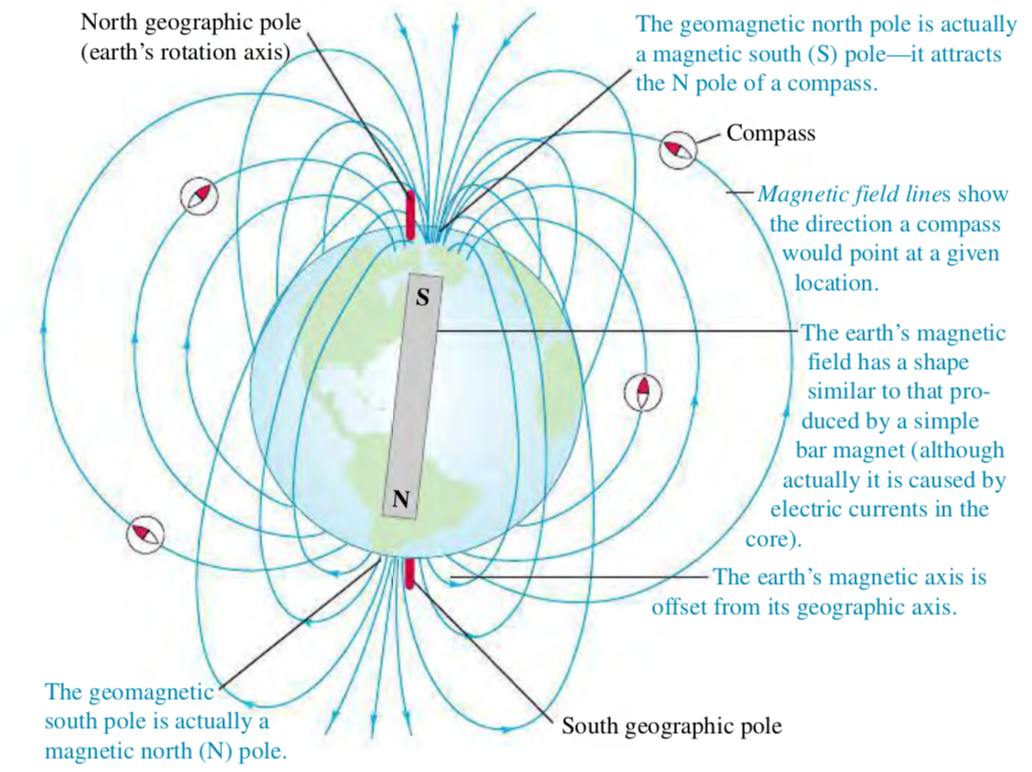
\includegraphics[scale=0.50]{images/earth's_poles.png}
\end{itemize}

\subsection{Magnetic Poles Versus Electric Charge}
\begin{itemize}
    \item While magnetic poles seem similar to positive and negative charges, they differ
        in that there is no evidence to suggest that one isolated magnetic pole can exist
    \item The existence of magnetic monopoles would have significant effects on
        theoretical physics
\end{itemize}

\section[27.2 Magnetic Field]{Magnetic Field}
\begin{itemize}
    \item A moving charge or current creates a magnetic field in the surrounding space
        (in addition to its electric field)
    \item The magnetic field exerts a force $\vec{\mathbf{F}}$ on the moving charge or
        current that is present in the field
    \item Like the Electric field $\vec{\mathbf{E}}$, the magnetic field
        $\vec{\mathbf{B}}$ is a vector field that points out of its north pole and into
        its south pole
\end{itemize}

\subsection{Magnetic forces on Moving Charges}
\begin{itemize}
    \item First characteristic of the magnetic force on a moving charge is that its
        magnitude is proportional to the magnitude of the charge
    \item The second characteristic is that the magnitude of the force is also
        proportional to the magnitude of the field
    \item The magnetic force also depends on the particle's velocity; this is quite
        different from the electric-force field, which is the same whether the charge is
        moving or not
    \item The fourth characteristic is that the magnetic force $\vec{\mathbf{F}}$ does
        not have the same direction as the field $\vec{\mathbf{B}}$ but is instead always
        perpendicular to both $\vec{\mathbf{B}}$ and $\vec{\mathbf{v}}$
    \item When $\vec{\mathbf{B}}$ and $\vec{\mathbf{v}}$ are parallel, the force is $0$
    \item The magnitude of $\vec{\mathbf{F}}$ is given by:
        \begin{equation}
            F = |q|v_{\perp}B = |q|vB\sin\phi
        \end{equation}
        where $|q|$ is the magnitude of the charge and $\phi$ is the angle measured from
        the direction of $\vec{\mathbf{v}}$ to the direction of $\vec{\mathbf{B}}$
    \item The equation to calculate $\vec{\mathbf{F}}$ is defined as:
        \begin{equation}
            \vec{\mathbf{F}} = q\vec{\mathbf{v}} \times \vec{\mathbf{B}}
        \end{equation}
    \item The direction of $\vec{\mathbf{F}}$ can be found using the right hand rule:

    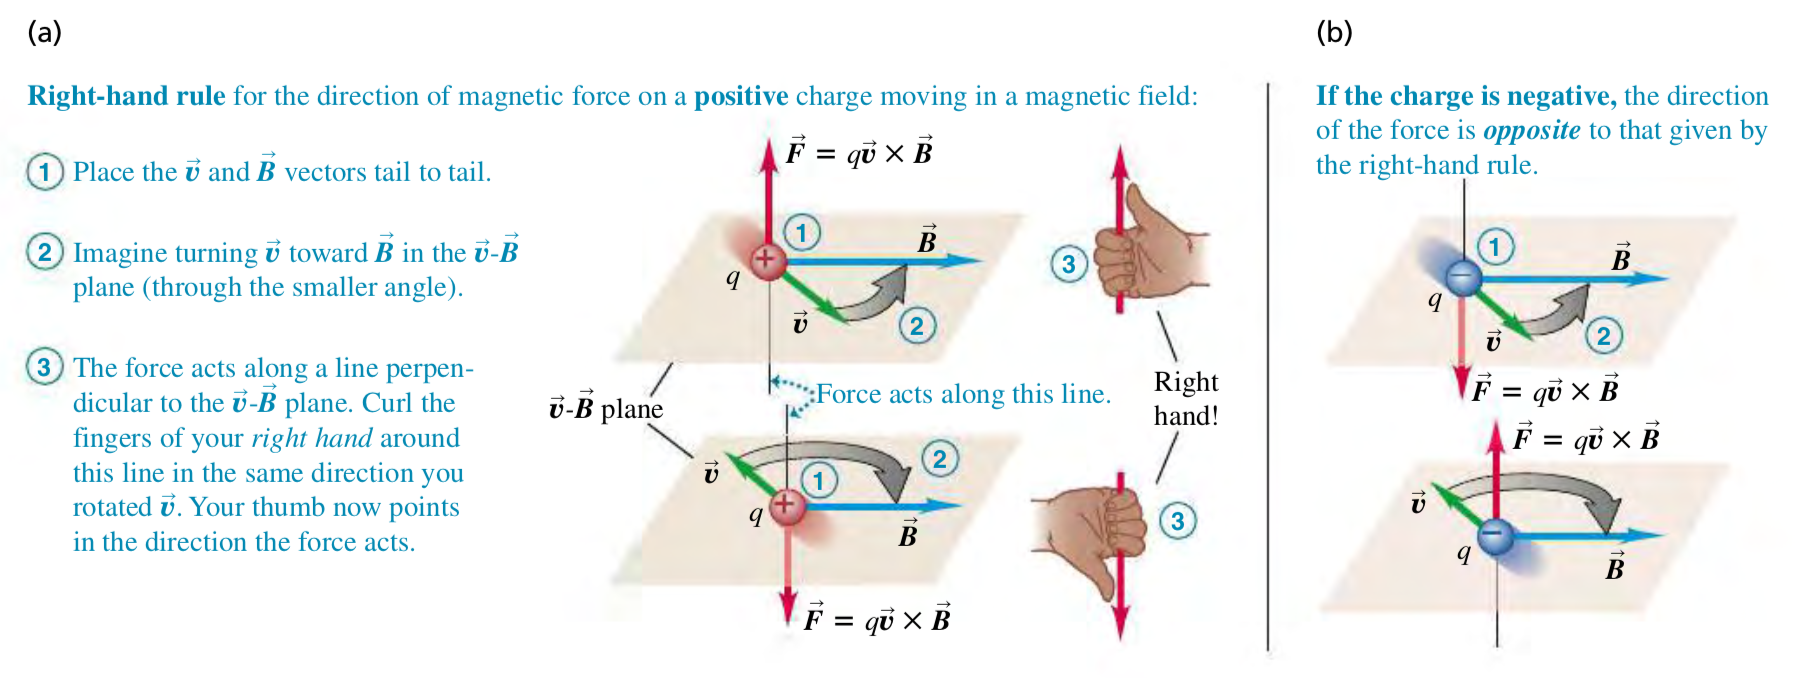
\includegraphics[scale=0.50]{images/right_hand_rule.png}

\end{itemize}

\subsection{Measuring Magnetic Fields with Test Charges}
\begin{itemize}
    \item To explore an unknown magnetic field, we can measure the magnitude and
        direction of the force on a moving test charge then calculate $\vec{\mathbf{B}}$
    \item When a charged particle moves through a region of space with both electric and
        magnetic fields, the total force $\vec{\mathbf{F}}$ is the vector sum of the
        forces:
        \begin{equation}
            \vec{\mathbf{F}} = q(\vec{\mathbf{E}} + \vec{\mathbf{v}}
            \times \vec{\mathbf{B}})
        \end{equation}
\end{itemize}

\section[27.3, Magnetic Field Lines and Magnetic Flux]{Magnetic Field Lines and Magnetic Flux}
Any magnetic field can be represented by magnetic field lines, where the more
dense the lines are in an area, the higher the magnitude of the magnetic field in
that location

\subsection{Magnetic Flux and Gauss's Law For Magnetism}
\begin{itemize}
    \item Magnetic Flux $\Phi_B$ through a surface in a similar fashion to electric flux
        with its connection to Gauss's law
    \item For each element $da$, determine $B_{\perp}$, the component perpendicular to
        $da$, altermatively, it can be written as $\vec{\mathbf{B}}\sin\phi = B_{\perp}$
    \item The Magnetic flux through an area $da$ is defined as:
        \begin{equation}
            d\phi_B = B_{\perp}dA = B\cos\phi dA = \vec{\mathbf{B}} \cdot
            d\vec{\mathbf{A}}
        \end{equation}
    \item The total magnetic flux through the surface is defined as:
        \begin{equation}
            \Phi_B = \int B\cos\phi dA = \int B_{\perp} dA = 
            \int \vec{\mathbf{B}} \mathbf{\cdot} d\vec{\mathbf{A}}
        \end{equation}
    \item This leads to Gauss's Law for magnetism:
        \begin{equation}
            \oint \vec{\mathbf{B}} \mathbf{\cdot} d\vec{\mathbf{A}} = 0
        \end{equation}
    \item Gauss's law always deals with closed surfaces, with $d\vec{\mathbf{A}}$
        pointing outwards
\end{itemize}

\section[27.4 Motion of Charged Particles in a Magnetic Field]{Motion of Charged
    Particles in a Magnetic Field}
\begin{itemize}
    \item The vectors $\vec{\mathbf{v}}$ and $\vec{\mathbf{B}}$ are perpendicular, so the
        magnetic force $\vec{\mathbf{F}} = q \mathbf{\vec{v} \times \vec{B}}$ has a
        magnitude $F = qvB$ 
    \item The force is always perpendicular to $\vec{\mathbf{v}}$, so it cannot change
        the magnitude, only the direction
    \item The centripetal acceleration is $v^2 / R$ and only the magnetic force acts, so:
        \begin{equation}
            F = |q|vB = m \frac{v^2}{R}
        \end{equation}
    \item Solving for $R$ yields:
        \begin{equation}
            R = \frac{mv}{|q|B}
        \end{equation}
\end{itemize}

\section[27.6, Magnetic Force On a Current Carrying Conductor]{Magnetic Force On a Current Carrying Conductor}
\begin{itemize}
    \item Can compute the force on a current-carrying conductor starting with the
        magnetic force $\vec{\mathbf{F}} = q \vec{\mathbf{v}} \times \vec{\mathbf{B}}$
    \item The drift velocity $\vec{\mathbf{v}}_d$ is upward, perpendicular to
        $\vec{\mathbf{B}}$. The average force of each charge is
        $\vec{\mathbf{F}}=q\vec{\mathbf{v}}_d \times \vec{\mathbf{B}}$ 
    \item The total force $\vec{\mathbf{F}}$ on all the moving charges in this segment
        has magnitude 
        \begin{equation}
            F = (nAl)(qv_{d}B) = (nqv_{d}A)(lB)
        \end{equation}
    \item The current density is given by $J = nqv_d$. With The total current $I$ equal
        to the product $JA$, so $F$ can be rewritten as:
        \begin{equation}
            F = IlB
        \end{equation}
    \item If $\vec{\mathbf{B}}$ is not perpendicular to the wire but forms an angle
        $\phi$ with it, the magnetic force is calculated as follows:
        \begin{equation}
            F = IlB_{\perp} = IlB\sin\phi
        \end{equation}
    \item The magnetic force vector can be calculated as follows:
        \begin{equation}
            \vec{\mathbf{F}} = I \vec{\mathbf{l}} \times \vec{\mathbf{B}}
        \end{equation}
    \item With the magnetic force on an infinitesimal wire segment being defined as:
        \begin{equation}
            d\vec{\mathbf{F}} = Id\vec{\mathbf{l}} \times \vec{\mathbf{B}}
        \end{equation}
\end{itemize}

\section[27.7, Force and Torque on a Current Loop]{Force and Torque on a Current Loop}
\begin{itemize}
    \item Looking at a rectangular current loop in a uniform magnetic field. We can
        represent the loop as a series of line segments
    \item The force $\vec{\mathbf{F}}$ on the right side of the loop (length a) is to the
        right. On this side, $\vec{\mathbf{B}}$ is the perpendicular to the current
        direction, and the force on this side has magnitude:
        \begin{equation}
            F = IaB
        \end{equation}

        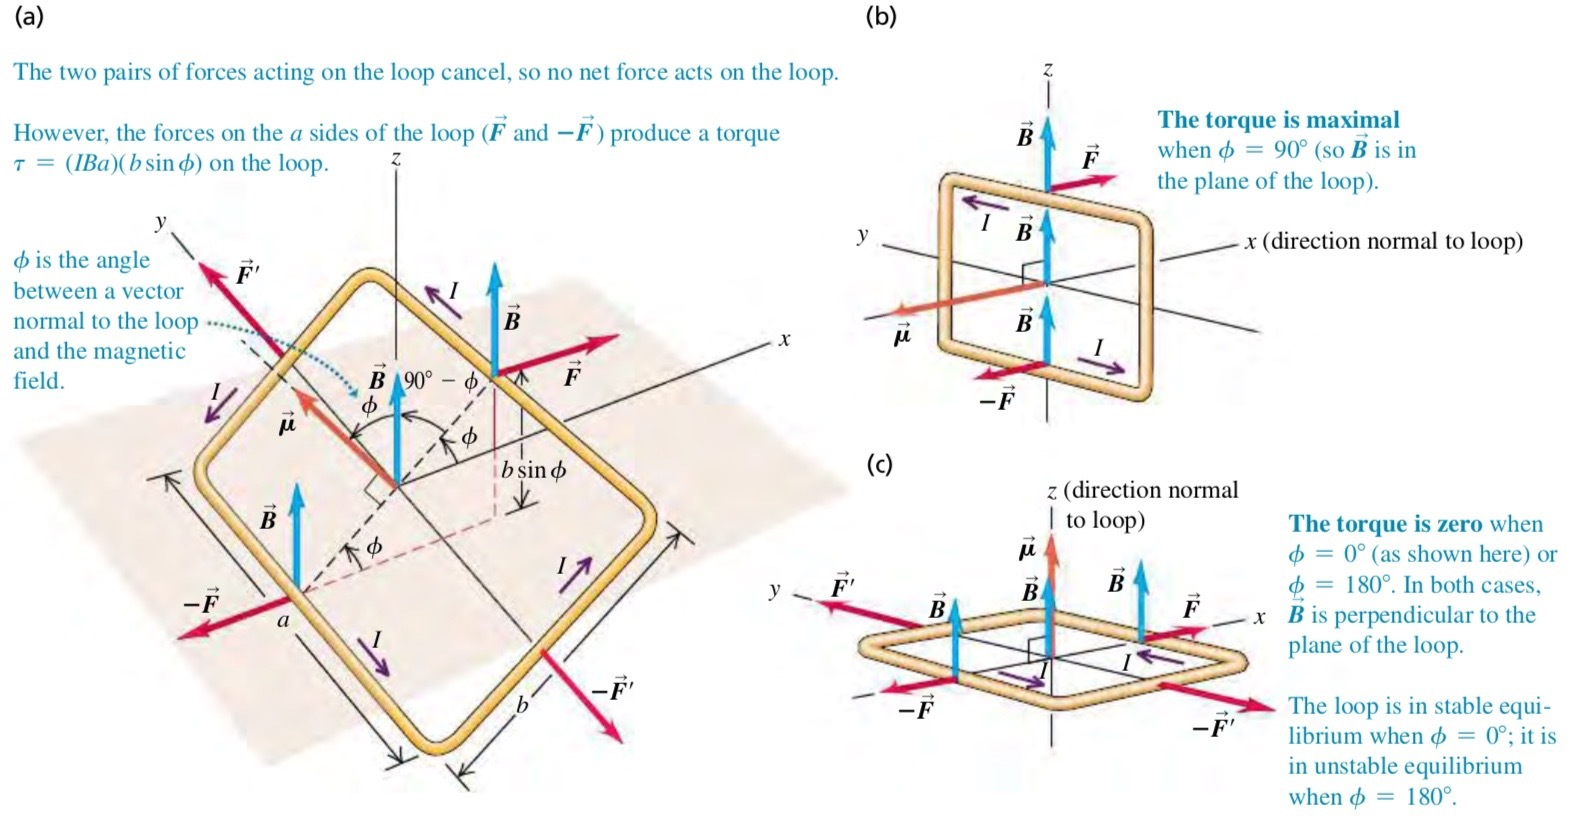
\includegraphics[scale=0.65]{images/square_current_loop.jpg}

    \item The net force on a current loop in a uniform magnetic field is zero. However,
        the net torque is not in general equal to zero
    \item The magnitude of the net torque is:
        \begin{equation}
            \tau = 2F(\frac{b}{2})\sin\phi = (IBa)(b\sin\phi)
        \end{equation}
    \item The torque is greatest when $\phi = 90^{\circ}$, $\vec{\mathbf{B}}$ is in the
        plane of the loop, and the normal to this plane is perpendicular to
        $\vec{\mathbf{B}}$
    \item Since the area A of the loop is equal to $ab$, the equation of torque can be
        rewritten as:
        \begin{equation}
            \tau = IBA\sin\phi
        \end{equation}
    \item The product $IA$ is called the \textbf{magnetic dipole moment} and is usually
        represented with $\mu = IA$
    \item The vector of magnetic torque can be represented as a cross product between the
        magnetic moment and the magnetic field:
        \begin{equation}
            \vec{\mathbf{\tau}} = \vec{\mathbf{\mu}} \times \vec{\mathbf{B}}
        \end{equation}
\end{itemize}

\end{document}
